In questo capitolo verranno mostrati gli esempi d'uso ed alcune dimostrazioni di come funzioni il servizio sviluppato.\\

Accedendo alla pagina iniziale, il servizio carica tutte le linee monitorate (per motivi di semplicità sono state usate solo quattro linee):
\vspace{1cm}
\begin{figure}[htbp]
\begin{center}
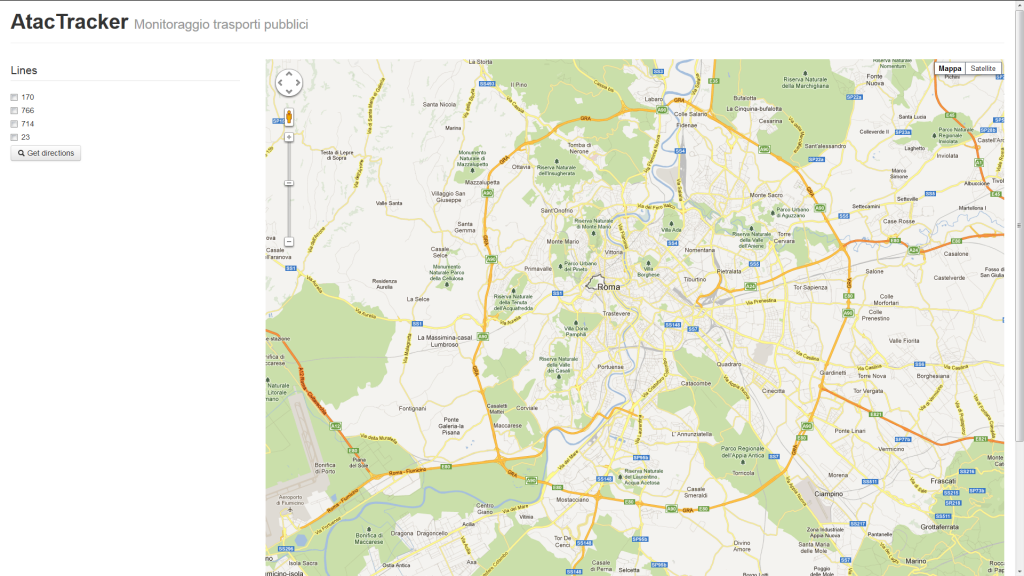
\includegraphics[width=13cm]{contents/images/home}
\end{center}
\caption{Pagina iniziale}
\label{fig:fermata}
\end{figure}

\newpage
Al momento della selezione delle linee scelte, il servizio prosegue richiedendo le direzioni appartenti a quelle linee per poi visualizzare all'utente, come si può constatare nella seguente figura:

\begin{figure}[htbp]
\begin{center}
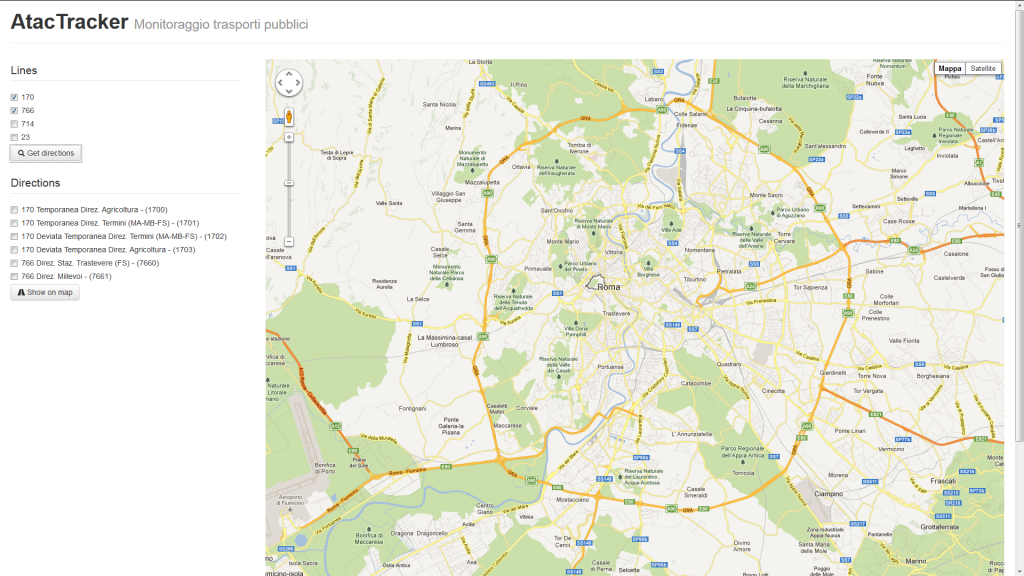
\includegraphics[width=13cm]{contents/images/directions}
\end{center}
\caption{Lista delle direzioni}
\label{fig:fermata}
\end{figure}

E' possibile notare come l'url sia composto dinamicamente in base alle scelte dell'utente, in base ai cambi di scelta che vengono richiesti, l'indirizzo viene assemblato con i giusti parametri:

\begin{figure}[htbp]
\begin{center}
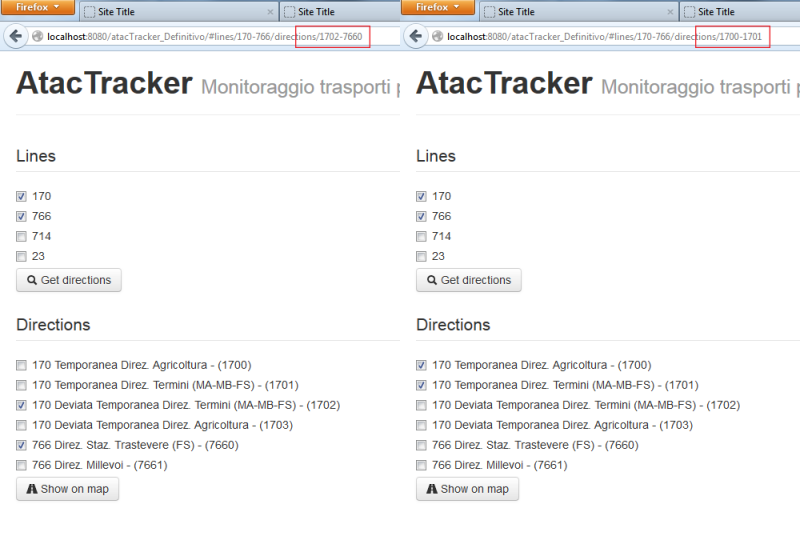
\includegraphics[width=12cm]{contents/images/indirizzo}
\end{center}
\caption{Modifica dinamica dell'url}
\label{fig:fermata}
\end{figure}
\newpage
Una volta selezionate le direzioni preferite e premuto l'apposito pulsante verranno visualizzate tutte le fermate inerenti a quelle direzioni e tutti gli autobus in circolazione presso quei tragitti, distinti tramite l'uso di marcatori di colore e forma differente.

Una semplice legenda aiuta l'utente a poter distinguere una direzione da un'altra:

\begin{figure}[htbp]
\begin{center}
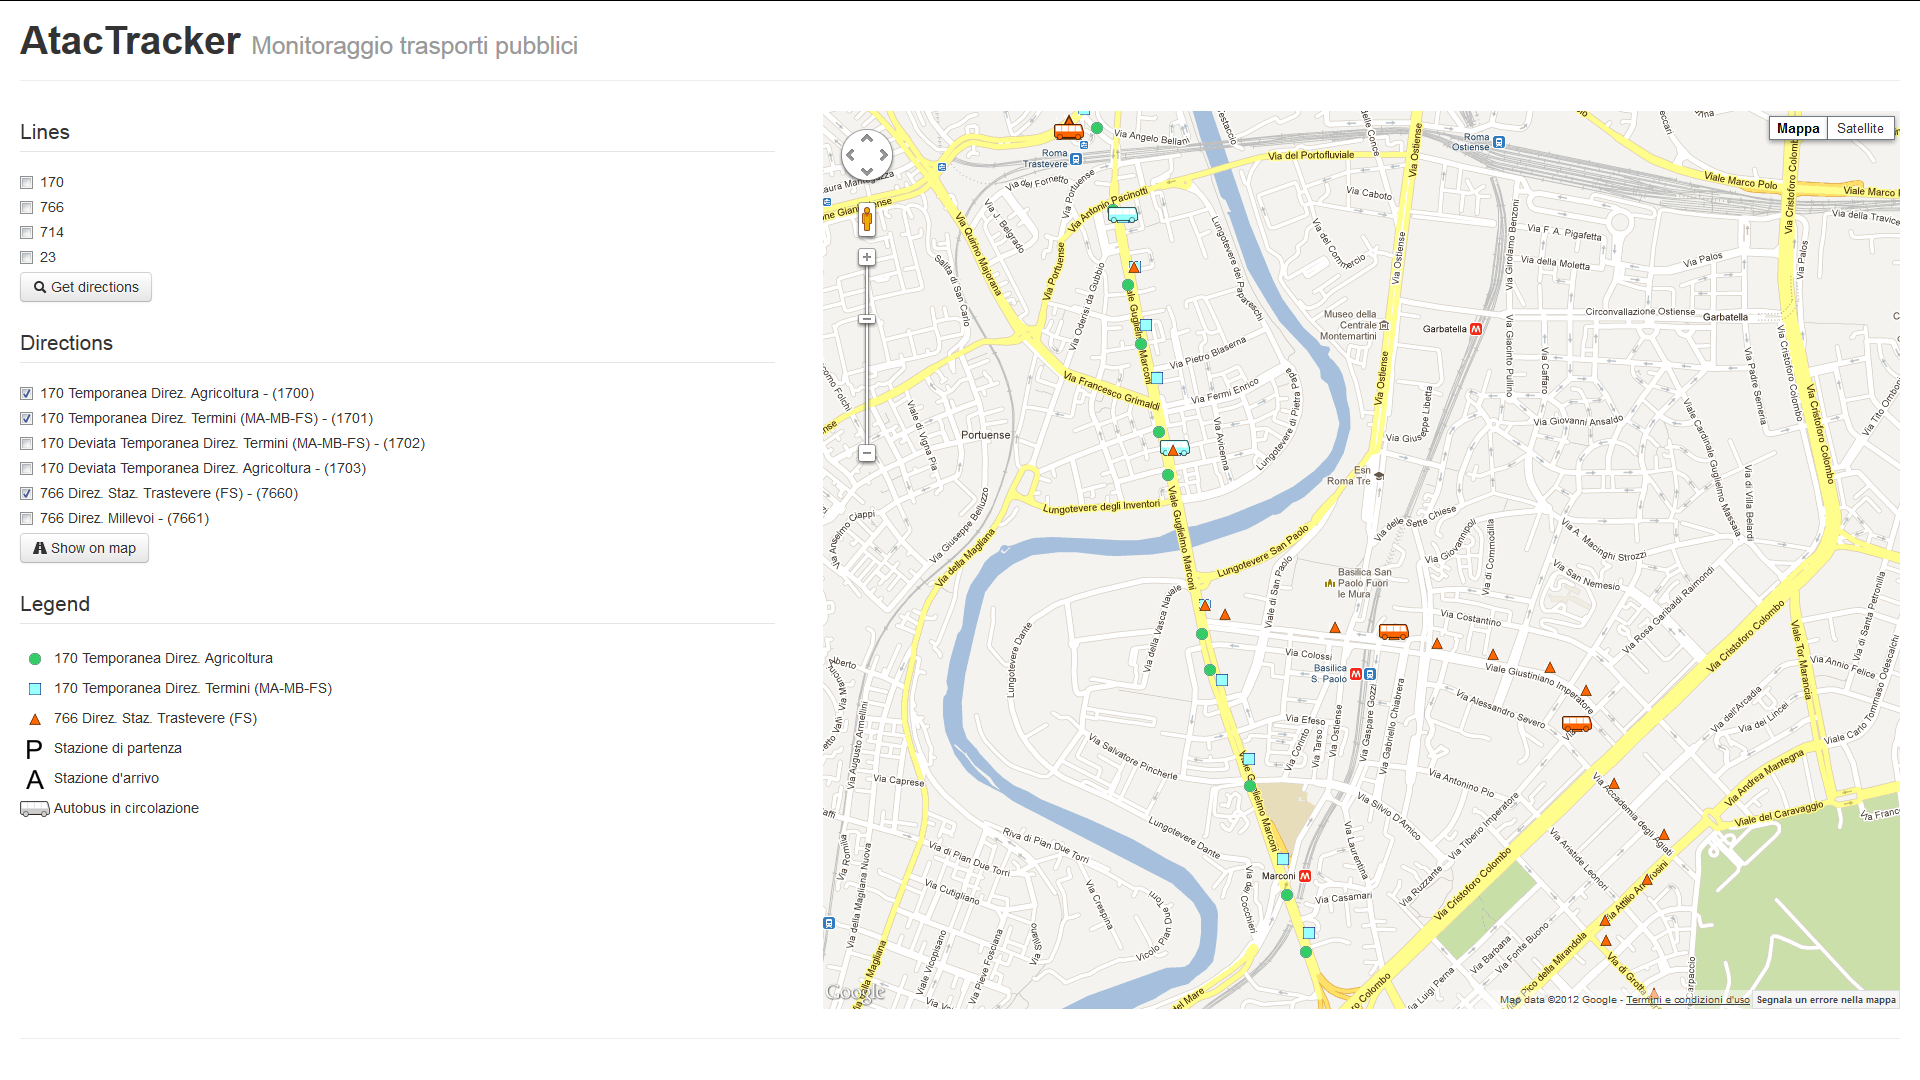
\includegraphics[width=13cm]{contents/images/bus}
\end{center}
\caption{Visualizzazione su mappa}
\label{fig:fermata}
\end{figure}

Col passare del tempo il servizio aggiornerà automaticamente la situazione degli autobus, aggiornando la mappa con le nuove posizioni:

\begin{figure}[htbp]
\begin{center}
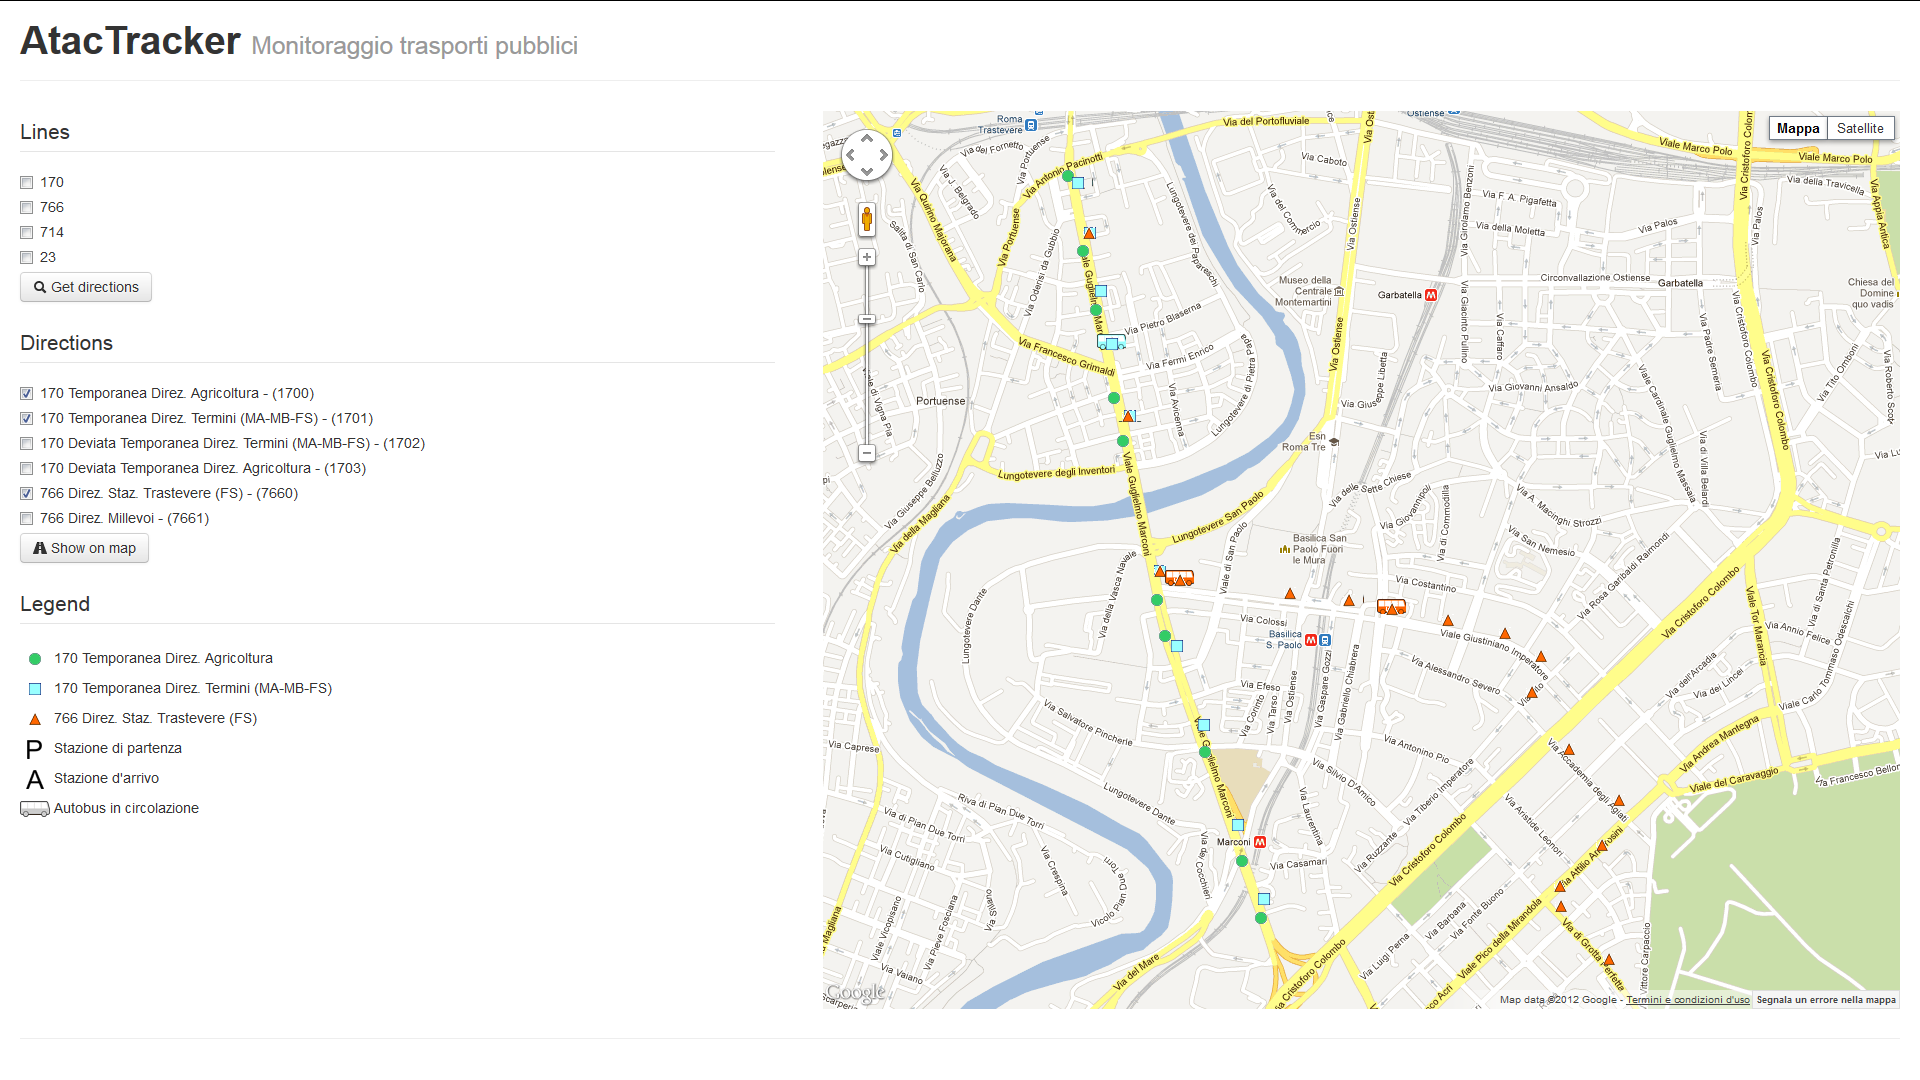
\includegraphics[width=13cm]{contents/images/bus2}
\end{center}
\caption{Visualizzazione dopo un minuto}
\label{fig:fermata}
\end{figure}
\newpage
Concludendo, si mostra come lo sviluppo di un sistema con Responsive Design permetta una corretta visualizzazione su qualunque dispositivo e qualunque risoluzione. Stringendo il browser, infatti, il sito si adatterà ai nuovi parametri di altezza e lunghezza, riposizionaro i vari elementi in modo opportuno:

\begin{figure}[htbp]
\begin{center}
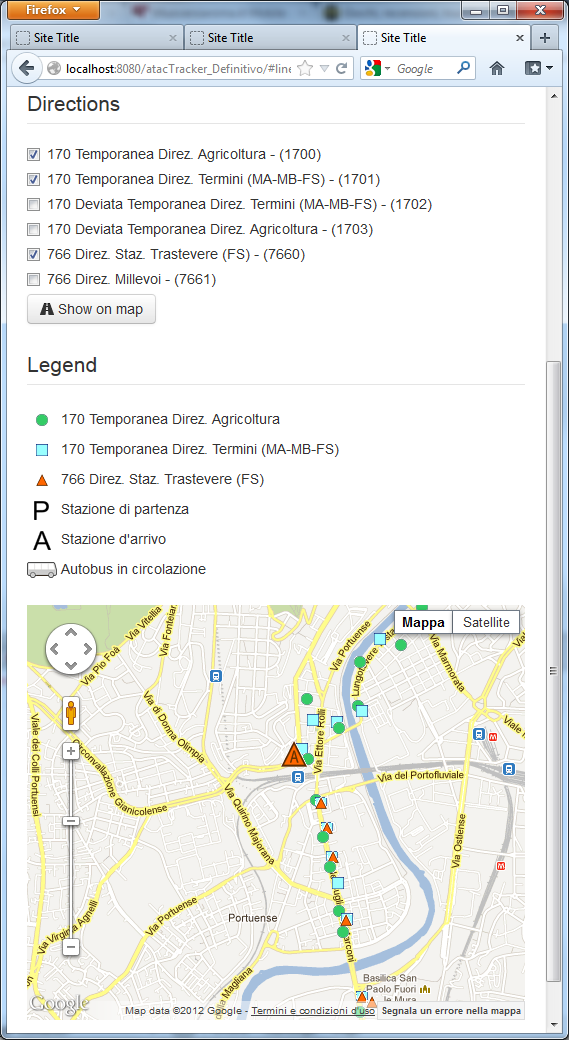
\includegraphics[height=15cm]{contents/images/responsive}
\end{center}
\caption{Visualizzazione con risoluzioni verticali}
\label{fig:fermata}
\end{figure}
